\documentclass{article}
\usepackage{aaai}
\usepackage{fixbib}
\usepackage{amsmath}
\usepackage{graphicx}
\usepackage{times}
\usepackage{helvet}
\usepackage{courier}
\usepackage{graphicx}
\usepackage{verbatim}
\usepackage{url}
\usepackage[utf8]{inputenc}
\DeclareUnicodeCharacter{FB01}{fi}
\graphicspath{ {images/} }
\frenchspacing
\setlength{\pdfpagewidth}{8.5in}
\setlength{\pdfpageheight}{11in}

\title{
	CS4246 AI Planning and Decision Making - Project 1 \\
	Depression Prediction
}
\author{
	{\bf Team 01} \\
	Antoine Charles Vincent Garcia - A0159072A\\
	Chan Jun Wei - A0112084U\\
	Chen Tze Cheng - A0112092W\\
	Eric Ewe Yow Choong - A0112204E\\
	Han Liang Wee, Eric - A0065517A\\
	Ho Wei Li - A0094679H\\
}

\begin{document}
 	\maketitle

	\begin{abstract}
	\begin{quote}
	Depression is a debiliatating mental illness that has good prognosis given early detection and treatment. 
	However, detection is difficult with the various factors that raise the entry barrier and decrease the accuracy of a diagnostic test. 
	In this study we aim to prove that prediction of depression severity on the PHQ-8 scale with voice acoustics is possible through the use of Gaussian Process, potentially lowering entry barriers to diagnostic tests and aiding early detection.
	\end{quote}
	\end{abstract}
	
	\section{Introduction}
	Depression has a severe, and at times long-term, negative impact on an individual's quality of life. 
	Major depression is 3rd leading cause of disability worldwide with 65 million life years spent living with the disability or lost due to early death \cite{who2004}.
	Depression's annual toll on U.S businesses amounts to about \$80 billion in medical expenditures, lost productivity and suicide. 
	Among the costs, close to \$10 billion accrued in lost workdays each year and more than \$33 billion in other costs accrue from decreased productivity due to symptoms that sap energy, affect work habits, cause problems with concentration, memory, and decision-making \cite{tjcp2015}. \\

	Left unchecked, depression increases risk for morbidity, suicide, decreased cognitive and social functioning, self-neglect, and early death \cite{arcp2009}. 
	Death from suicide is one of the top 10 causes of death, above the death rate for chronic liver disease, Alzheimer's, homicide, arteriosclerosis or hypertension \cite{nvsr2016}. \\

	Despite the severe consequences, depression is one of the most treatable mental illnesses but it is also one of the most under-diagnosed globally. 
	In general health-care, 48.4\% of patients suffering from depression go unrecognized \cite{jama2003}.

	\subsection{Motivation and Objective}
	The Personal Health Questionaire depression scale (PHQ-8) is a self-administered, 8-question diagnostic test for depressive disorders that has proven to be an effective severity measure for depression in large clinical studies \cite{jad2008}. 
	Nevertheless, one of the biggest obstacles to successful diagnosis of depression is the unwillingness of patients to admit their predisposition to depression by seeking help.\\

	People often subscribe to the social stigma that being depressed reflects a weakness in their character, a permanent defect in their personality. 
	This stigma manifests itself particularly in a phenomenon known as social distancing whereby people with mental issues are more isolated from others \cite{tpcrp2011}.  
	People suffering from depression hence tend to be ashamed of their condition and are generally convinced that denying and hiding it from others gives them a better shot at integrating with society and living a normal life \cite{bmb2001}.
	 Even if they do seek help, the accuracy of the PHQ-8 or just questionaires and surveys in general are often adversely affected by the Hawthorne Effect, a type of reactivity in which individuals modify or improve an aspect of their behavior in response to their awareness of being observed. \cite{jce2014}. \\

	In the past decade, there have been research successfully correlating emotion with voice production and speech acoustics \cite{uwa2001}. 
	Corollary to that, active research of late into the use of voice acoustics as predictors of clinical depression scores has seen some success, proving that it is an effective indicator of depression severity \cite{jov2016}. \\

	The aim of the present study is to determine if acoustic measures of voice, characterizing specific spectral and timing proerties, predict predetermined clinical ratings of depression severity on the PHQ-8 scale in a sample of patients, using an existing dataset of their voice recordings. \\
	
	\subsection{Future Applications}
	Findings from this experiment will reinforce results from similar experiments and make a stronger case for the possibility of lowering the entry barriers of depression diagnostic tests and at the same time, increasing the accuracy of depression diagnosis by abstracting the Hawthorne Effect. 
	Diagnostic tests can be designed in a friendly way that does not require the patient to consciously answer questionaires such as the PHQ-8 or even to have complete awareness of the diagnostic process. 
	By taking into account the Hawthorne Effect and the status quo of the social stigma and working around them, diagnoses can be made easier, faster and more accurately and with that, education and treatment can begin early before the mental condition of the patient deteriorates. \\
	
	\section{Modelling and Approach}
	As Gaussian Process Regression Model is a new state of the art machine learning model, we are trying to apply it for depression prediction 
	with the hope that the accuracy of depression prediction will be improved. \\	
	
	The following assumptions have been made for the experiment so that the GP Regression Model is suitable for depression prediction:
	\begin{enumerate}
		\item For any depressed individual, it is possible to identify depression via his/her speech. \cite{Cummins2015}
		\item Depression Prediction is an event-based recognition which provides a single depression estimates over a certain amount of time. \cite{Valstar2016}
		\item The speech signals extracted from different depressed people should share some similarities and thus suitable for prediction with the Gaussian Process Model. 
		For example, a diminished prosody and monotonous and “lifeless” sounding speech is indicative of depression.\cite{Cummins2015}
	\end{enumerate}

	\subsection{Qualitative Advantages}
	GP is exceptionally useful in this application as it enables us to perform prediction on various training data including outliers or 
	those with irregular sampling rates. As our assumption of we are able to determine of depressed person according to the speech and all 
	the signals extracted share some similarities, we could make use of the training data in GP to perform prediction for a depressed person based on the speech of the person.\\

	With GP, we can obtain a probability distribution such as the predictive mean and variance. 
	These properties have a significant role to play in estimating the depression levels. For instance, 
	the mean could be use as the baseline for an average working-human mood. The variance here would give us a picture to how good our existing data is. 
	So, if some area of the probability distribution gives very high variance, it means that we don’t have enough data for that area. 
	Therefore, using the properties of GP we could determine how well our database is and we can find out what is the average depression level for 
	everyone in the world nowadays. \\

	In addition, GP produces truly probabilistic outputs with an explicit degree of prediction uncertainty. 
	The prediction uncertainty can be further analyse to produce useful results. In addition, there exist algorithms for GP hyperparameter 
	learning—something the other Machine Learning methods like SVM framework lacks. It is very useful as hyperparameter estimation could provide 
	improvement to the Machine Learning algorithm especially in sound/speech recognition. \cite{Hashimoto2015} \\

	Previously,  SVM gave a very high accuracy of prediction in speech emotion recognition, scoring about 94 \% 
	of accuracy in classification of emotions. \cite{Chavhan2010}. However, in a more recent research, GP actually beats SVM in emotion recognition. 
	In the paper  “Music Genre and Emotion Recognition Using Gaussian Processes“ \cite{MARKOV2013}, 
	both music genre classification and music emotion estimation tasks, the GP performed consistently better than the SVM. \\

	Therefore, as we are trying to prediction on depression, we would like to use GP to process our data to produce a more accurate prediction result. 
	
	\subsection{Requirements}\label{audio_feats}
	Aside from the audio recordings, our GP model makes use of the following:
	\begin{enumerate}
		\item \textbf{Audio Features}	\\
		What are the differences between sounds? To differentiate between sounds, we need to learn about audio features, which will be described below:
		\begin{enumerate}
			\item \textbf{Energy}	\\
			The Energy feature of a sound refers to the loudness of the sound at various timeframes, 
			hence it is obvious that energy of a sound is directly proportional to the amplitude of the soundwave. 
			This shows that the higher the energy, the louder the sound is going to be.	
		
			\item \textbf{Mel Frequency Cepstral Coefficients (MFCC)} \\
			Mel Frequency Cepstral (MFC) is a representation of short-term power spectrum of a sound, 
			based on a linear cosine transform of a log power spectrum on a nonlinear Mel scale of frequency. 
			The greatest benefit of using MFCC is that the scale approximates the 
			human's auditory system response more closely, hence it allows for a better representation of sound. 
			In order to obtain MFCC, Fourier transform is performed on the sound signals.	
		
			\item \textbf{Magnitude Spectrum} \\
			Magnitude spectrum can be produced by converting the input signal of an audio into frames. 
			Fast Fourier Transform (FFT) is performed on each frames and this will form the Magnitude Spectrum.
			
			\item \textbf{Zero-Crossing Rate} \\
			Zero crossing rate is the rate of sign-changes along a signal. This feature is extremely useful in speech recognition and music information retrieval.
		\end{enumerate}
		
		\item \textbf{Kernels}	\\
		The similarity measure of all features is usually called kernel. As Gaussian Process uses Kernels to predict the value for an unseen point from training data, 
		understanding different kernels that we are going to use is extremely useful. \\
		The kernels that would we are intested in is shown below 
		(The kernels are assumed to be defined on two samples \( x = ( x_{1} x_{2} x_{3} ... x_{n} ) \) and 
		\( x' = ( {x_{1}}' {x_{2}}' {x_{3}}' ... {x_{n}}')\) ,  
		represented as feature vectors in some input space):
		\begin{enumerate}
			\item \textbf{Radial Basis Function (RBF)}\\
			The RBF kernel is defined as 
			\begin{equation}\label{eq:kernel_rbf}
				K(x,x') = \exp^{-\frac{||x-x'||^{2}}{2\sigma^{2}}}
			\end{equation}
			\(||x-x'||^{2}\) represents Squared Euclidean Distance 
			And \( \sigma > 0 \) can either be a scalar (isotropic variant of the kernel) or a vector with the same number of dimensions 
			as the inputs X (anisotropic variant of the kernel). \\
			It is also known as the squared exponential kernel. This kernel is infinitely differentiable, 
			which implies that GPs with this kernel as covariance function have mean square derivatives of all orders, 
			and are thus very smooth.
			
			\item \textbf{Matern}\\
			The class of Matern kernels is a generalization of the RBF and the absolute exponential kernel parameterized 
			by an additional parameter nu. The smaller the value of nu, the less smooth the approximated function is. For nu=\(\infty\), 
			the kernel becomes equivalent to the RBF kernel and for nu=0.5 to the absolute exponential kernel. 
			Important intermediate values are nu=1.5 (once differentiable functions) and nu=2.5 (twice differentiable functions).

			\item \textbf{Automatic Relevance Detection (ARD) Kernels}\\
			If we chose the anisotropic variant of the RBF and Matern kernel, then these kernels would be also called as ARD kernels. 
			So, what it means for the model is, (let's assume the numbe of dimensions of the input is N) for each \(\sigma_{i}\), where i = 1,2,3,...,N, 
			might be different, depending the importance of the corresponding input features. \\

			ARD is advantageous for the experiment such that: \cite{Cawley2014}
			\begin{enumerate}
				\item Generalisation performance is potentially improved.
				\item The data would be better explained.
				\item Increase the efficiency of feature extraction for audio.
			\end{enumerate}
			
			\item \textbf{Dot Product}\\
			The Dot Product kernel is non-stationary and can be obtained from linear regression by putting N(0, 1) priors on the coefficients 
			of \(x_{d}\) (d = 1, . . . , D) and a prior of N(0, \(\sigma_{0}^{2}\)) on the bias. 
			The Dot Product kernel is invariant to a rotation of the coordinates about the origin, but not translations. 
			It is parameterized by a parameter \(\sigma_{0}^{2}\). For \(\sigma_{0}^{2} = 0\), 
			the kernel is called the homogeneous linear kernel, otherwise it is inhomogeneous. The kernel is given by
			\begin{equation}\label{eq:kernel_dp}
				K(x,x') = \sigma_{0}^{2} + x \cdot x'  
			\end{equation}
		\end{enumerate}

		While Matern is a very generalized kernel, both isotropic and ARD variant of the Matern kernel is selected for our model. 
		On the other hand, as dot product kernel is a very efficient and simple kernel, 
		we decide to give it a try too. \\
		As we favor simplicity, we actually think that dot product kernel would give us the best result.
	\end{enumerate}

	\subsection{Machine Learning Methods Applied}
	Machine learning is about using models to learn from existing data for some improvement or predictions. 
	The following is some methods used in machine learning:
	\begin{enumerate}
		\item \textbf{k-nearest neighbors algorithm} \\
		The k-Nearest Neighbors algorithm is a non-parametric method for classification and regression. 
		The training examples are vectors in a multidimensional feature space, each with a class label. 
		The data will be classified into the class with most number of occurrence within the defined k radius.
	
		\item \textbf{Support Vector Machines (SVM)} \\
		Support Vector Machine (SVM), with the help of the libsvm, is a type of linear classifiers that aims at finding 
		a unique solution in the form of an optimal hyperplane which is defined as the one that maximizes the margins between the two classes.

		\item \textbf{Random Forest Regressor} \\
		Random Forest is an ensemble of decision trees, whereas a decision tree tries to separate the data into different leaf nodes 
		where the data points in each node have certain similarity. Each decision tree will predict a value and the values will be averaged to be the result.
	
		\item \textbf{AdaBoost} \\
		AdaBoost is the short form of Adaptive Boost which is sensitive to noisy data and outliers. 
		AdaBoost first find out the classifier with the least errors, adding the weight to the outliers, then find out another classifier with least errors again.
		A final classifier will be combined and indicate the class of data.
	
		\item \textbf{Naive Bayes} \\ 
		Naive Bayes is a prediction algorithm that uses Bayes rule. 
		All naive Bayes classifiers assume that the value of a particular feature is independent of the value of any other feature, given the class variable. 
		The possibilities is represented by the number of times the particular event occurs in the dataset over the total number of events. 
	\end{enumerate}

	\subsubsection{Hypothesis: Doing feature selection before applying to the ARD Kernel Gaussian Process model will improve the result.}
	Without doing feature selections, as the feature dimensions would be huge, we would also have large number of kernel parameters. 
	As a result, it is likely to lead to overfitting and generating poor result. \cite{Cawley2014} 
	Thus, to increase the effectiveness of the Gaussian Process Model, we would apply feature selection to the data first.

	\subsubsection{Hypothesis: MFCC is the most important feature.}
	Depression is actually tied to emotions : it can either mean sadness or people who deny feeling sad. \cite{Stratou2015} 
	On the other hand, as the baseline accuracy of using only MFCC to predict emotions is quite high, \cite{ElAyadi2011}, 
	we actually guess that MFCC is the most important feature in depression prediction. 
	In other words, since we have limited datas and large feature dimension, 
	using MFCC feature only for the input vector of the model might actually improve the result. \\

	\section{Evaluation}
	In order to test our proposed Gaussian Process models, we conducted tests on data obtained from Audio/Visual Emotion Challenge and Workshop(AVEC 2016) 
	\cite{avec2016}. The goal of AEVC is to weigh-in on the various approaches(visual, audio) used to recognize emotions under unambiguous conditions. 
	AVEC 2016 provided 2 pieces of data as input: visual and auditory data from each of the participants. However, we would be reducing the scope of 
	the experiment, limiting the experiment to only the auditory data. Two Sub-Challenges were lised in AVEC 2016. We are only interested in the Depression Classification Sub-Challenge, which 
	requires participants to classify inputs by the PHQ-8 score.
	
	In this experiment, we would be using the audio data along with their corresponding PHQ-8 to test our hypotheses.

	\subsection{Data}
	\begin{figure}[h]
	\center
 	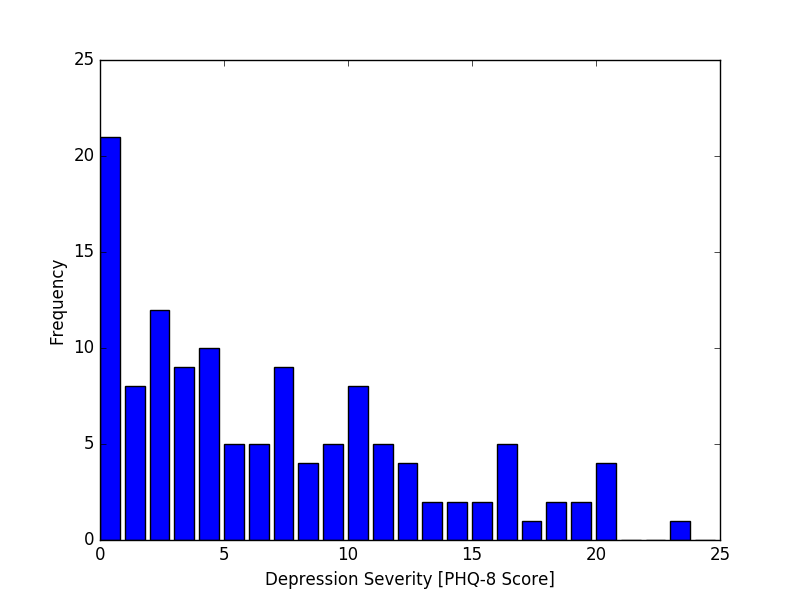
\includegraphics[width=0.35\textwidth]{histogram_phq8}
	\caption{Histogram of the PHQ-8 scores}
	\label{histogram_phq8}
	\end{figure}
	
	The depression data used in AVEC 2016 was obtained from the benchmarking database, the Distress Analysis Interview Corpus - Wizard of Oz (DAIC-WOZ). 
	Data collected from DAIC-WOZ include raw audio and video recordings and the corresponsing PHQ-8 score(from 0 to 24)\cite{jad2008}. Hence, we would 
	need to pre-process the auditory data before we use it in our experiment. The pre-processing is briefly discussed in the section below.
	The distribution of the depression severity scores in the dataset is given in Figure \ref{histogram_phq8}. The data provided are split into 2 sets: training and development.
	A summary of the data is given in Table \ref{summary_table}.

 	\begin{table}[h]
 		\begin{center}
  			\begin{tabular}{ | r | c | c || c | }
    			\hline
			 & Training & Development & All \\ \hline\hline
			 n               & 95 & 31 & 126 \\ \hline
			 $\mu$           & 6.326 & 7.548 & 6.626 \\ \hline
			 $\sigma$        & 5.597 & 6.690 & 5.909 \\ \hline
			 \end{tabular}
		\end{center}
 	\caption{Summary of Datasets provided}
 	\label{summary_table}
 	\end{table}

    \subsection{Pre-processed data}
	Since the focus of this paper is the prediction of the PHQ-8 score, we will not describe the pre-processing step in detail.
	We used standard signal processing techniques to extract the 4 audio features (Energy, MFCC, Magnitude Spectrum, Zero-crossing) as presented in section above titled Audio Features.
	Each audio features is composed of several individual features, the breakdown of the actual number of feature columns are as follows.

 	\begin{table}[h]
 		\begin{center}
  			\begin{tabular}{ | r | c | }
    			\hline
			 Audio Feature & Number of features \\ \hline\hline
			 Magnitude Spectrum               & 512 \\ \hline
			 MFCC           & 12 \\ \hline
			 Energy        & 1 \\ \hline
			 Zero-Crossing Rate & 1 \\ \hline \hline
			 Total & 526 \\ \hline
			 \end{tabular}
		\end{center}
 	\caption{Number of features extracted}
 	\label{no_features}
 	\end{table}

 	\subsection{Measure of Accuracy}
	AVEC 2016 provided a baseline classifier that consistently predicts the PHQ-8 score with $\text{RMSE}=6.7418$\cite{avec2016}. 
	In order to provide a meaningful and consistent comparison to the baseline provided, we would also use Root Mean Square Deviation Error (RMSE) to measure the error rate on both 
	Training and Development datasets. RMSE(Equation \ref{eq:rmse}) is a commonly used in machine learning communities to measure the differences between the values predicted by a model 
	and the ground truth\cite{Dhanani:EECS-2014-131}. 
	\begin{equation}\label{eq:rmse}
  	\text{RMSE} = \sqrt{\frac{\sum_{t=1}^n (\hat y_t - y_t)^2}{n}}
 	\end{equation} 

	\subsection{Feature Selection}
	Feature selection is the process of selecting a subset of relevant features including variables or predictors to be used in a model construction for machine learning. 
	The usage of feature selection is to reduce the complexity of a model in machine learning to be interpreted easier. 
	The objective of variable selection is three-fold: improving the prediction performance of the predictors, providing faster and most cost-effective predictors, 
	and providing a better understanding of the underlying process that generated the data. \cite{Guyon2003} Since we have more features than data points, it leads to overfitting\cite{Smith2011}. We would
	 need to perform feature selection on the data before using the machine learning algorithm.
	 
	The litany of feature selection algorithms used are popular and are taken from scikit-feature, a feature selection library\cite{li2016feature}: CIFE\cite{Lin2006}, reliefF\cite{Rob2003}, CFS\cite{HALLHALL}. We will not go into detail as feature selection is not the main focus of the report.
	
	\subsection{Experimental Setup}
	We compared the proposed Gaussian Models against commonly used machine learning algorithms as mentioned in the previous section. For the ease of testing, all implementations of the algorithms except for GP ARD come from the popular machine learning library, Scikit Learn\cite{scikit-learn}. We used the 
	implementation of GP ARD from GPy, a Gaussian Processes framework in Python\cite{gpy2014}.
	The hyper-parameters are either determined by the defaults used in either libraries or some reasonable defaults were used.
	Each machine learning algorithm is trained against the training set and thereafter tested against the development set using RMSE as the error metric. 
	The entire experimental process is shown in Figure \ref{process}.
 
 	\begin{comment}
	\begin{table}[h]
  		\begin{center}
   			\begin{tabular}{ | r | c |}
	    		\hline
			Algorithm & Hyper-parameters \\ \hline\hline
			K-Nearest Neighbors        & x \\ \hline
			SVM - Linear               & x \\ \hline
			SVM - RBF                  & x \\ \hline
			Decision Tree              & x \\ \hline
			Random Forest              & x \\ \hline
			AdaBoost                   & x \\ \hline
			Naive Bayes                & x \\ \hline
			GP ARD  	           & x \\ \hline
			GP Isotropic Matern        & x \\ \hline
			GP Dot Product 	           & x \\ \hline
			\end{tabular}
		\end{center}
		\caption{List of Machine Learning Algorithms with their corresponding hyper-parameters}
		\label{list_mls}
	\end{table}
 	\end{comment}
 	
	\begin{figure}[h]
 		\begin{center}
		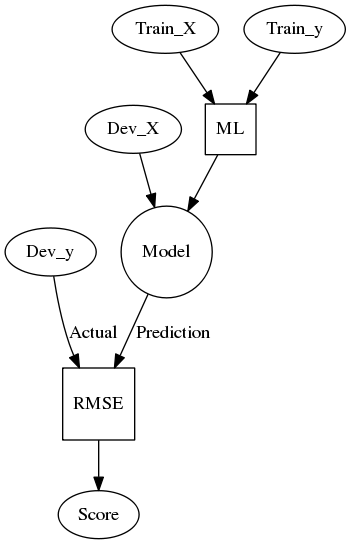
\includegraphics[width=0.45\textwidth]{process} 
  		\end{center}
  		\caption{Experimental process}
  		\label{process} 
 	\end{figure}
 	\begin{comment}
	@startuml
	digraph g {
		graph [rankdir=LR];
	 	ML,RMSE[shape=square];
		Model[shape=circle];
		ap[shape=rect label="Audio Processing"];
		Train_AudioData,Dev_AudioData[shape=egg];
		Train_AudioData -> ap;
		ap -> Train_X;
		ap -> Train_y;
		ap -> Dev_X;
		Dev_AudioData -> ap;
		ap -> Dev_y;
		Train_X -> ML;
		Train_y -> ML;
		ML -> Model
		Dev_X -> Model
		Model -> RMSE[label=Prediction]
		Dev_y -> RMSE[label=Actual]
	}
	@enduml
 	\end{comment}

	\subsection{Results}
	We first run the experiment across the dataset across all 526 features, without feature selection. As we would expect\cite{Cawley2014}, the results are terrible as the number of features is more than the number of 
	data points, potentially
	 causing overfitting. The results of the experiment is illustrated in figure \ref{results_all}. We would expect the GP ARD would be able to theoritcally extract relevant features and improve
	  prediction. However, we have seen experimentally that GP ARD performs poorly, along with other GPs. The results for all the features are shown in figure \ref{rmse_results}.

	\begin{figure}[h]
 		\begin{center}
		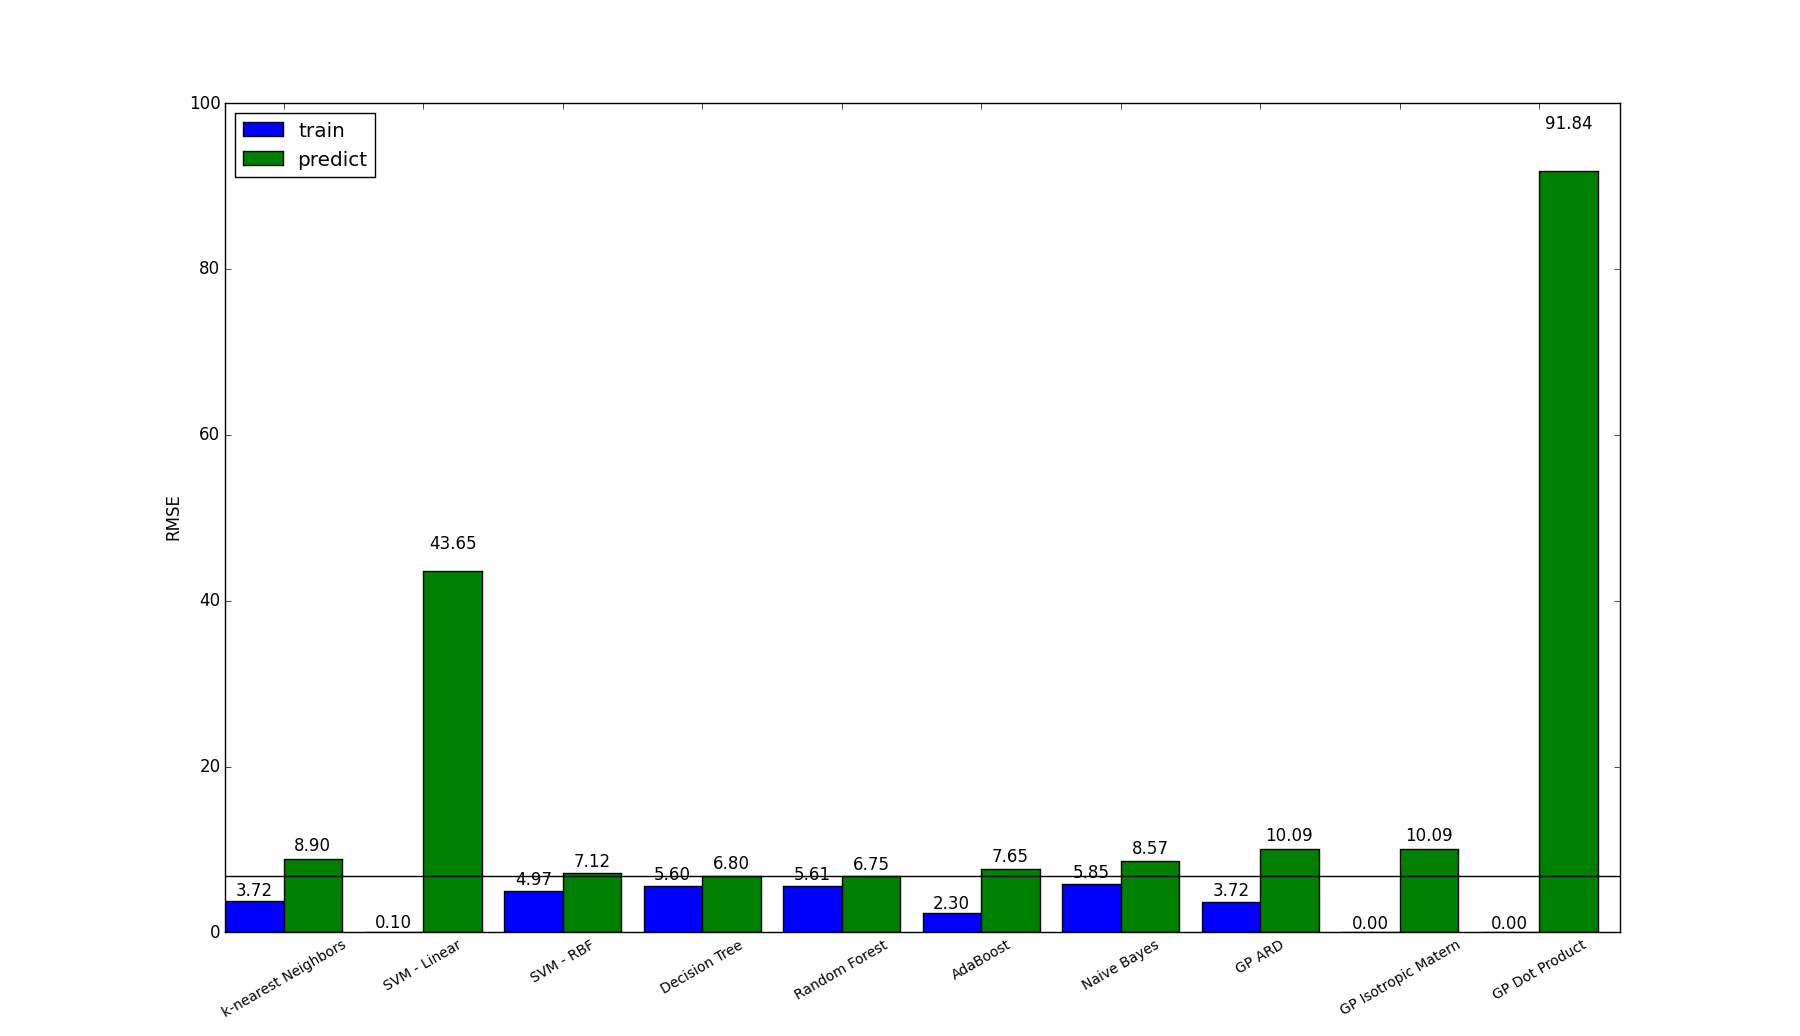
\includegraphics[width=0.45\textwidth]{results_all} 
  		\end{center}
  		\caption{Results across all features}
  		\label{results_all}
 	\end{figure}
	
	We re-run the experiment across the data with feature selection. We run each of the feature subset gathered from the feature selection algorithms against each of the machine learning algorithm. 
	We observe that reliefF, CIFE and CFS selected a large number of MFCC features. This confirms our hypothesis that MFCC gives the best predictive power to predict PHQ-8. Hence, in addition we also ran 
	the experiment on MFCC features, and are represented as MFCC alongside the feature subsets obtained from feature selection. The best results across all feature subsets are shown in figure \ref{results_best} and in table \ref{rmse_results}. 

	\begin{figure}[h]
 		\begin{center}
		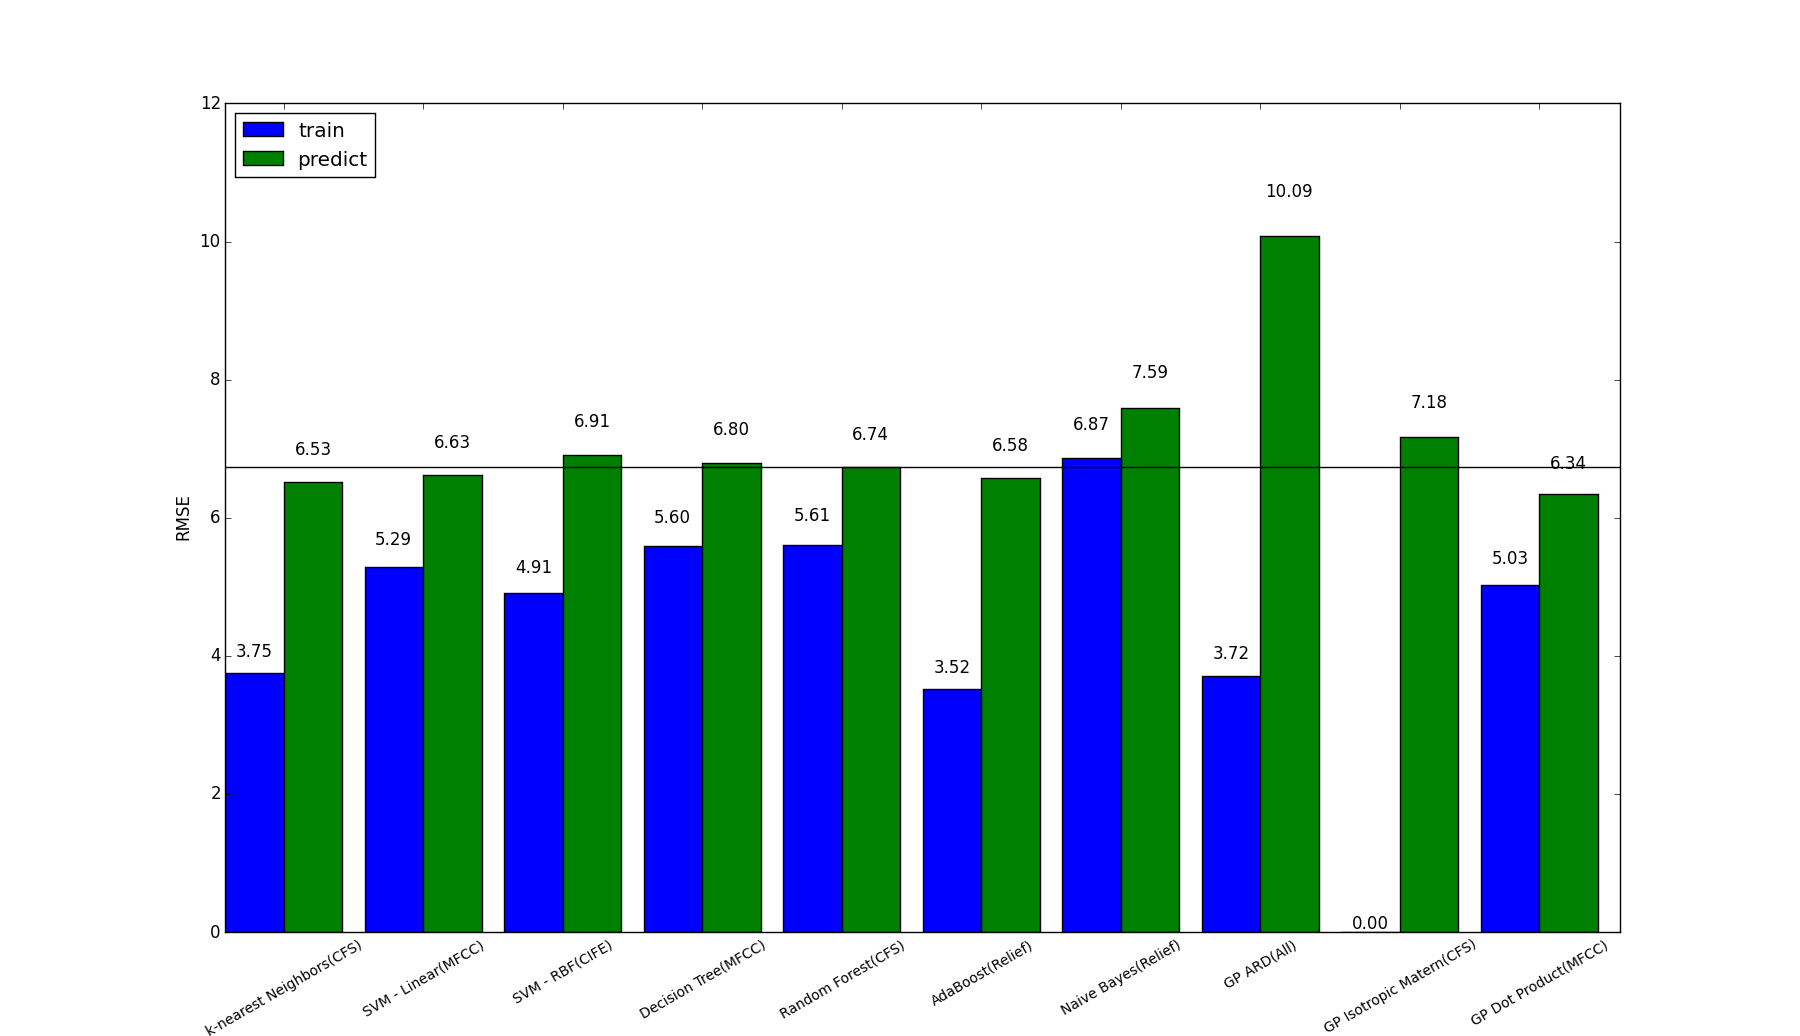
\includegraphics[width=0.45\textwidth]{results_best} 
  		\end{center}
  		\caption{Best Results across all feature subsets}
  		\label{results_best}
 	\end{figure}

	\begin{table}[h]
		\begin{center}
			\begin{tabular}{ | r | c | c | c | }
			\hline
			&& \multicolumn{2}{c|}{RMSE} \\ \hline
			Algorithm 		   & Subset& Train & Dev \\ \hline\hline
			K-Nearest Neighbors        & x & x \\ \hline
			SVM - Linear               & x & x \\ \hline
			SVM - RBF                  & x & x \\ \hline
			Decision Tree              & x & x \\ \hline
			Random Forest              & x & x \\ \hline
			AdaBoost                   & x & x \\ \hline
			Naive Bayes                & x & x \\ \hline
			GP ARD                     & x & x \\ \hline
			GP Isotropic Matern        & x & x \\ \hline 
			GP Dot Product             & x & x \\ \hline
			\end{tabular}
		\end{center}
		\caption{RMSE results of the different machine learning algorithms}
		\label{rmse_results}
	\end{table}

	\section{Conclusion}	
	Our work has succesfully modelled the various levels of depression with GP by taking audio recordings as our input. \\
	
	\section{Contributions}
	\begin{itemize}
		\item \textbf{Antoine Charles Vincent Garcia}: 
		Scripting the program, setting up machine learning libraries and running tests.
		\item \textbf{Chan Jun Wei}: 
		Project technicalities such as problem formulation and modelling, mathematics and experiment planning.
		\item \textbf{Chen Tze Cheng}: 
		Project technicalities such as problem formulation and modelling, mathematics and experiment planning.
		\item \textbf{Eric Ewe Yow Choong}: 
		Formatting of the report, resolution of LaTeX issues and keeping track of requirements
		\item \textbf{Han Liang Wee, Eric}: 
		Scripting the program, setting up machine learning libraries and running tests.
		\item \textbf{Ho Wei Li}: 
		Background research and writing up of the abstract and introduction section with its subsections.
	\end{itemize}
	
	\newpage
	\bibliographystyle{aaai}
	{\scriptsize \bibliography{references}}

\end{document}
